\chapter{Introduction}
\section{Overview}
Traditional methods of analyzing timeseries images produced by 
\ac{fMRI} perform regression using the linear combination of explanatory variables. 
Though adding degrees of freedom naturally mandates more computation,
in this thesis I will demonstrate the use of the Particle Filters to 
estimate the governing parameters of the \ac{BOLD} model at a computation cost 
that would still allow real time calculations for multiple voxels.
More practically, this method is an alternative
method of detecting neural activity from the traditionally
used \ac{SPM}. Though more computationally intense,
this method is capable of modeling nonlinear effects, is conceptually simpler
and provides more detailed output. Additionally,
by using a separate particle filter for each single time series it 
is possible to estimate parameters and make real-time predictions
for small neural regions, a feature which could be useful towards real time \ac{fMRI}
\cite{DeCharms2005}. Future works will also benefit from the ability to 
apply conditions to the posterior distribution in post-processing without
recalculating parameters; for instance, to impose additional 
physiological
constraints. Modeling the \ac{BOLD} response 
as a nonlinear system is the
best way to determine the correlation of a stimulus sequence with the \ac{BOLD}
response; yet in the past doing this on a large scale has been far too
computationally taxing. The solution used here takes approximately 40 seconds
for a single 5 minute time series (with Core 2 Duo Q6600). 

This thesis is organized as follows. The introduction will introduce
\ac{BOLD}, the method by which neural time changing data is detected. This section
will also describe the basic form of the \ac{BOLD} model - which drives the 
detectable changes in \ac{MR} signal. \autoref{sec:Prior Works} will discuss other
methods of analyzing \ac{fMRI} images as well as other techniques that have
been, or could be applied to the nonlinear regression model described here. 
\autoref{sec:Particle Filter} derives the particle filter using Bayesian 
statistics and discusses some practical elements of implementing the 
particle filter algorithm. \autoref{sec:Methods} then goes into further
detail about the specific particle filter configuration used in this work.
This section also describes the pre-processing pipeline. 
The results are described separately for simulated data
and real \ac{fMRI} data in \autoref{sec:SimulationResults} and \autoref{sec:RealData},
respectively. In \autoref{sec:Discussion} the results and their implications
are further discussed. Future improvements to this technique, as well
as applications are then explored in \autoref{sec:FutureWork}.
Finally in \autoref{sec:Conclusion} the significant findings and 
impact of this work are reviewed. 

\section{Historic Context}
\acresetall
For the past twenty years, \ac{fMRI}
has been at the forefront of cognitive research. Despite its
limited temporal resolution, \ac{fMRI} is the standard tool for localizing 
neural activation.  Whereas other methods
of analyzing neural signals can be invasive or difficult to acquire, 
\ac{fMRI} is simple to setup quick and inexpensive.
By modeling the governing equations behind the neural response that
drives \ac{fMRI}, it is possible to increase the power of \ac{fMRI}.
The underlying state equations hold important information
about how individual brain regions react to stimuli. The model parameters
on the other hand, hold important information about the patients individual
physiology including existing and future pathologies. In short,
the long chain of events driving \ac{fMRI} signals contain information 
beyond correlation with stimuli.

In the past fifteen years, a steady stream of studies have built
on the original \ac{BOLD} signal 
derivation first described by Ogawa et al. \cite{Ogawa}.
The seminal work by Buxton et al. attempted to explain the
time evolution of the \ac{BOLD} signal using a windkessel model to
describe the local changes in \ac{dHb} content \cite{Buxton1998}.
Incremental improvements were made to this model until Friston et al.
brought all the changes together into a single complete 
set of equations \cite{Friston2000}. While there have been numerous adaptations in the model, 
many of them summarized by Deneux et al., even the basic versions
have less bias error than the empirically driven Canonical \ac{HRF}
\cite{Deneux2006,Handwerker2004}.
On the other hand \ac{BOLD} signal models have numbers
of parameters ranging from seven \cite{Riera2004} to 50 \cite{Behzadi2005} 
for a signal as short as 100 samples long. This number of parameters presents
a significant risk of being under-determined and having high computation cost. 
In this work, only the simplest physiologically inspired model will be
used (with 7 parameters), and steps will be taken to make the most of computation
time.

\section{Overview}
\label{sec:Introduction Overview}
Detecting neural activity using the changes in \ac{fMRI} images is based on 
the \ac{BOLD} signal.
The \ac{BOLD} signal is caused by minute changes in the ratio of 
\ac{dHb} to \ac{O2Hb} in blood vessels throughout the brain \cite{Ogawa}.
Because \ac{dHb} is paramagnetic, higher concentrations
attenuate the signal detected during \ac{T2}-weighted \ac{MRI}
techniques. The most common \ac{fMRI} imaging technique, due to its rapid 
\ac{TR}, is \ac{EPI}. When axons become active,
large amounts of ions quickly flow out of the cell. In order for this
action potential to occur again (and thus for the neuron to fire again),
an active pumping process must move ions back into the
axon. This process of recharging the axon requires extra energy, which temporarily
increases the metabolic rate of oxygen. On a massive scale (cubic millimeter) 
this activation/recharge process happens continuously. However, when a 
particular region of the brain is significantly active, the action potentials
occur more often, resulting in a local increase of the 
\ac{CMRO2}. Thus, if everything else 
stays the same, blood vessels in an active area will 
tend to have less \ac{O2Hb}, and more \ac{dHb}
(due to the increased rate at which oxygen is being consumed).
This would then result in an attenuated \ac{fMRI} signal. However, to
compensate for activation, muscles that
control blood vessels relax allowing increased blood flow,
which actually overcompensates.
This ultimately results in lower than average concentration of 
\ac{dHb}. Thus, the \ac{BOLD} signal consists of a short initial
dip in the \ac{MR} signal, followed by a prolonged increase in signal
that slowly settles out. It is the overcompensation that provides
the  primary signal detected with \ac{fMRI}. This cascade of events
is believed to drive a prolonged increase in local metabolism, 
blood flow, blood volume, and \ac{O2Hb}. The differences
in onsets and recovery times of these variables are what cause the 
distinguishing characteristics of the \ac{BOLD} signal. Unfortunately, 
\ac{fMRI} signal levels are all relative: within a particular
person, scanner and run. 

\begin{figure}
\centering
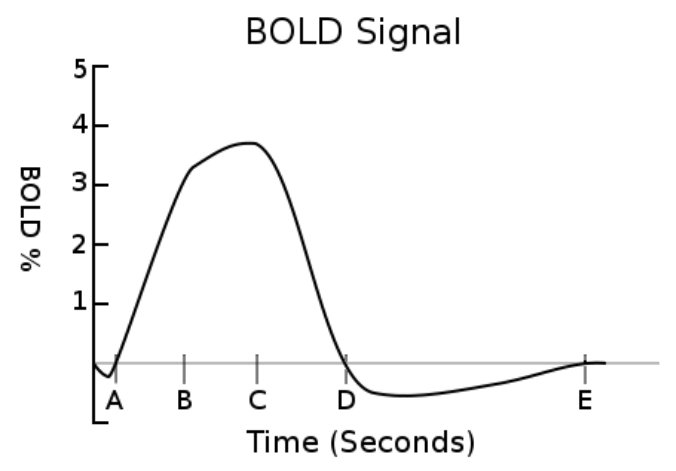
\includegraphics[width=.5\textwidth]{images/bold2}
\caption[Diagram of \ac{BOLD} Signal]{Diagram of the \ac{BOLD} Sigmal.
A) End of Pre-Stimulus Undershoot, $< 2s$ typical,
B) End of Stimulus, C) Input Bloodflow Drops from Supernormal to Subnormal,
$5 s$ after B typical, D) Beginning of Post-stimulus Undershoot, $12 s$ after B
typical, E) Full return to normal, between $20-30s$ after B.}
\end{figure}

\section{Functional Magnetic Resonance Imaging}
\ac{MRI}, is a method of building 3D images
non-invasively, based on the difference between nuclear spin
relaxation times in different molecules. The technique is
well established and documented in various works \cite{Bushberg2002}. 
First, the subject 
is brought into a large magnetic field which causes nuclear spins
to align. \ac{RF} signals may
then be used to excite nuclear spin away from the base alignment. 
As the nuclei precess back to the alignment of the magnetic
field, they emit detectable \ac{RF} signals. Conveniently, the
nuclear spins return their original state at different
rates, called the \ac{T1} relaxation time, depending on the material excited.
Additionally, the
coherence of the spins also decays differently (and roughly an order of 
magnitude faster
than \ac{T1} relaxation) based on the properties of the region 
\cite{Bushberg2002}.
This gives two primary methods of contrasting substances,
which form the basis of \ac{T1} and \ac{T2} weighted images. Additionally, 
dephasing occurs at two different rates, the \ac{T2} relaxation time,
which is unrecoverable, and \ac{T2}$^*$ relaxation, which is
much faster, but possible to recover from via special \ac{RF} signals.
\ac{T1} relaxation times are typically on the order of seconds if 
a sufficiently strong excitation is applied, whereas \ac{T2}$^*$ relaxation
times are usually less than 100ms. 
In order to rapidly acquire entire brain images, as done in Functional 
\ac{MRI}, a single large excitation pulse is applied to the entire brain,
and the entire volume is acquired in a single \ac{T1} relaxation period
\cite{Obata2004}. 
Because the entire k-space (spatial-frequency) volume is acquired 
from a single excitation, the \ac{SNR} is very low
in \ac{EPI} \cite{Smith2007}. 

Increasing the spatial resolution of \ac{EPI} necessarily 
requires more time or faster magnetic field switching. Increasing
switching rates can result in
more artifacts and lower signal to noise ratios. The result is
that at best \ac{fMRI} is capable of 1 second temporal resolution
\cite{Ladd2010, Poser2010}. 
The signal is also diluted because each voxel contains
a variety of neurons, capillaries and veins \cite{Obata2004}. 
Thus, the \ac{fMRI} signal, which is sensitive to the chemical composition of 
materials, is the average signal from various types of tissue
in addition to the blood. As mentioned in \autoref{sec:Introduction Overview},
and explored in depth in \autoref{sec:BOLD Physiology},
the usefulness of \ac{fMRI} comes from discerning changes in 
\ac{dHb}/\ac{O2Hb} \cite{Ogawa, Obata2004}. Therefore, it is necessary to assume
that the only chemical changes will be in
capillary beds feeding neurons. In practice this may not be the case, for
instance near large veins, and it may explain some of the
noise seen in \ac{fMRI} imaging (see \autoref{sec:Introduction Noise}). 
Because \ac{MRI} is unitless and certain
areas will have a higher base \ac{MR} signal, all \ac{fMRI} studies deal with
percent change from the base signal; rather than raw values. 

\section{BOLD Physiology}
\label{sec:BOLD Physiology}
It is well known that the two types of \ac{Hb} act as contrast agents in 
\ac{EPI} imaging \cite{Buxton1998, WEISSKOFF1994, Ogawa}, however the connection
between \ac{dHb}/\ac{O2Hb} and neural activity is non-trivial. 
Intuitively, increased 
metabolism will increase \ac{dHb}, however blood vessels are quick
to compensate by increasing local blood flow. Increased inflow, accomplished by loosening 
capillary beds, precedes increased outflow, driving increased 
blood storage.
Since the local \ac{MR} signal depends on the ratio of \ac{dHb} to \ac{O2Hb},
increased blood volume affects this ratio if 
metabolism doesn't exactly match the increased inflow of oxygenated blood.
This was the impetus
for the ground breaking balloon model \cite{Buxton1998} and windkessel
model \cite{Mandeville1999}. These works derive, from first principals,
the changes in \ac{dHb} ratio and volume of capillaries given an inflow waveform.
These were the first two attempts to quantitatively account for the shape of the 
\ac{BOLD} signal as a consequence of the lag between the \ac{CBV}
and the inward \ac{CBF}. 

Although Buxton et al. demonstrated that a well chosen flow waveform could 
explain most features of the \ac{BOLD} signal, it stopped short of proposing a
realistic waveform for the \ac{CBF} and \ac{CMRO2} \cite{Buxton1998}. Friston et al. 
gave a reasonable and simple
expression for \ac{CBF} input based on a flow inducing signal
and in the same work proposed a simple method
of estimating metabolic rate: as a direct function of the inward blood flow \cite{Friston2000}.
By combining these equations with the balloon model from Buxton et al.,
it is possible to predict the \ac{BOLD} signal directly from a stimulus time course:
\begin{eqnarray}
\dot{s} &=& \epsilon u(t) - \frac{s}{\tau_s} - \frac{f - 1}{\tau_f} \\
\dot{f} &=& s\\
\dot{v} &=& \frac{1}{\tau_0}(f - v^\alpha)\\
\dot{q} &=& \frac{1}{\tau_0}(\frac{f(1-(1-E_0)^f)}{E_0} - \frac{q}{v^{1-1/\alpha}})
\label{eq:bold}
\end{eqnarray}
where $s$ is a flow inducing signal, $f$ is the input \ac{CBF},
$v$ is normalized \ac{CBV}, and $q$ is the normalized
local \ac{dHb} content. The 
parameters controlling blood flow are $\epsilon$, which is a neuronal 
efficiency term, $u(t)$ which is the stimulus, and $\tau_f$, $\tau_s$ 
which are time constants. The parameters for the evolution of blood 
volume are $E_0$ which the resting metabolic
rate and $\alpha$ which is Grubb's parameter controlling the balloon model. 
$\tau_0$ is a single time constant controlling the speed of $v$ and $q$.

This completed balloon model was assembled and analyzed
by Riera et al. \cite{Riera2003}. Obata refined the readout equation 
of the \ac{BOLD} signal based on the
\ac{dHb} content (q) and local blood volume (v), resulting in the
final \ac{BOLD} equation \cite{Obata2004}.
\begin{eqnarray}
y   &=& V_0((k_1 + k_2)(1-q) - (k_2 + k_3)(1-v))\\
k_1 &=& 4.3 \times \nu_0 \times E_0 \times TE = 2.8\\
K_2 &=& \epsilon_0 \times r_0 \times E_0 \times TE = .57\\
k_3 &=& \epsilon_0 - 1 = .43
\label{eq:boldout}
\end{eqnarray}
Where $\nu_0 = 40.3 s^{-1}$  is the frequency offset in Hz for fully
de-oxygenated blood (at 1.5T), $r_0 = 25 s^{-1}$  is the slope relating
change in relaxation rate with change in blood oxygenation, $TE$ is the
echo time used by the \ac{EPI} sequence and $\epsilon_0 = 1.43$ is the 
ratio of signal \ac{MR} from intravascular to extravascular regions at rest. Although,
these constants change with experiment ($TE$, $\nu_0$, $r_0$),
patient, and brain 
region ($E_0$, $r_0$), often the estimated values by Obata are 
taken as the constants $a_1 = k_1 + k_2 = 3.4$, and $a_2 = k_2+k_3 = 1$ in 
studies using 1.5 Tesla scanners \cite{Obata2004}.
While this model is more accurate than the static hemodynamic model used in \ac{SPM},
there are other additions which give it more degrees of freedom. 

\section{Post Stimulus Undershoot}
\label{sec:Post Stimulus Undershoot}
Although the most widely used, the \ac{BOLD} model described in \autoref{eq:bold}
and \autoref{eq:boldout} has been extended in various fashions. The most
significant feature missing from the original model is the 
post-stimulus undershoot.
The post-stimulus undershoot is the term used for a prolonged subnormal
\ac{BOLD} response for a period of 10 to 60 seconds after stimulus has
ceased \cite{Chen2009,Mandeville1999a}.

Because \autoref{eq:bold} is not capable of producing such a prolonged undershoot,
additional factors must be present. Two prominent theories exist to explain the post 
stimulus undershoot.  Recall
that a lower than base signal means that there is an increased \ac{dHb}
content in the voxel. The first and simplest explanation is that the post-stimulus
undershoot is caused by a prolonged increase in \ac{CMRO2} after \ac{CBV} and \ac{CBF}
have returned to their base levels. This theory is justified by 
studies that show \ac{CBV} and \ac{CBF} returning to the baseline before the \ac{BOLD} signal
\cite{Frahm2008, Donahue2009, Buxton2004, Lu2004, Shen2008}. 
Unfortunately, because of limitations on \ac{fMRI} and in vivo
\ac{CBV}/\ac{CBF} measurement techniques it is difficult to isolate whether \ac{CBF} and
\ac{CBV} truly have returned to their baseline. Other studies indicate
that there can be a prolonged supernormal \ac{CBV}, although none of these papers completely
rule out the possibility of increased \ac{CMRO2}  \cite{Mandeville1999a,
Behzadi2005, Chen2009}. The discrepancies may in part
be explained by a spatial dependence in the post-stimulus undershoot; described
by Yacoub et al. \cite{Yacoub2006}. In Chen et al. 
a compelling case is made that most of the post stimulus undershoot can be 
explained by combination of a prolonged \ac{CBV} increase, and a prolonged \ac{CBF} 
undershoot \cite{Chen2009}. Additionally it was proposed that
the previous measurements showing a quick recovery of \ac{CBV} 
were in fact showing a return to baseline by arterial \ac{CBV} (which
has little effect on the \ac{BOLD} signal).

Regardless of the probability that \ac{CMRO2} and \ac{CBF} are detached,
research into the post-stimulus undershoot has led to the creation
of much more in depth models. In Zhen et al. additional state
variables model oxygen transport, whereas Buxton et al. models
\ac{CMRO2} from a higher level, and somewhat more simply; though it 
still adds 9 new parameters \cite{Zheng2002, Buxton2004}. Behzadi et al. 
introduced nonlinearities into the \ac{CBF} equations as a method to
explain the post-stimulus undershoot, which falls in line with a 
prolonged increase in \ac{CBF} observed by Chen et al. \cite{Behzadi2005, Chen2009}. 
Similarly Zheng et al. added additional compartments for 
venous and arterial blood \cite{Zheng2005}. 
Deneux et. al. compared these models and though 
that work did not deal extensively with the 
post-stimulus undershoot, it did show incremental improvements
in quality from the additional parameters \cite{Deneux2006}.  
Importantly, Deneux et al. did show that by 
simply adding viscoelastic terms from Buxton et al. a slowed return 
to baseline is possible to model, without greatly increasing
complexity \cite{Deneux2006, Buxton2004}. Regardless, because these models are more 
complex, and the parameters are not well characterized, in this work the simple
Balloon model is used. 

In summary, there have been extensive refinements to the Balloon
model; however, the increased complexity and lack of known priors 
make these models difficult to work with. Additional degrees of freedom 
could also make parameter estimation intractable.

\section{Properties of the Blood-Oxygen-Level Dependent Model}
\label{sec:BOLD Analysis}
Since the first complete \ac{BOLD} model was proposed by Friston et al. 
\cite{Friston2000},  
several studies have analyzed its properties.  
The most important property is that the system is dissipative, and given
enough time will converge to a constant value. This is found simply by
analyzing the eigenvalues of the state equation Jacobian, 
\cite{Deneux2006, Hu2009}. The steady state of the Balloon
model equations gives:

\begin{eqnarray}
s_{ss} &=& 0 \nonumber \\
f_{ss} &=& \tau_f\epsilon u + 1\nonumber \\
v_{ss} &=& (\tau_f\epsilon u + 1)^\alpha\nonumber \\
q_{ss} &=& \frac{(\tau_f\epsilon u + 1)^\alpha}{E_0}(1-(1-E_0)^{1/(\tau_f\epsilon u + 1)})\nonumber \\
y_{ss} &=& V_0((k_1+k_2)(1-q_{ss}) - (k_2+k_3)(1-v_{ss}))
\label{eq:steadystate}
\end{eqnarray}

where the parameters are all the same as in \autoref{eq:bold}

In real \ac{fMRI} data, there is a significant nonlinearity in response; with short sequences
responding disproportionately strongly \cite{Birn2001, Wager2005, Deneux2006}.
This nonlinearity is accounted for in the Balloon model, although Deneux et al.
showed that when duration of stimuli varies greatly,
modeling Neural Habituation is necessary to fully capture the range of responses \cite{Deneux2006}. 
Both Birn et al. and Deneux et al. found that 
stimuli lasting longer than 4 seconds 
tend to be more linear, which is why block designs are so well accounted for
by the \ac{GLM} (see \autoref{sec:Current Techniques General Linear Model})
\cite{Birn2001, Deneux2006}.

Another interesting result from Deneux et al. was the sensitivity analysis \cite{Deneux2006}.
That work found that the parameters are far from perpendicular,
and that very different parameters could give nearly identical \ac{BOLD} output.
The means that that without constraining parameter values, they may not be 
precisely ascertainable. This could explain discrepancies of parameter estimates
in previous studies (\autoref{tab:Params}).

%note to self, friston2002b's parameters are from a picture
\begin{table}[t]
\centering
\begin{tabular}{|c || c | c | c | c|}
\hline 
Parameter  & Friston et al. \cite{Friston2000} & Jonston et al. \cite{Johnston2007} 
    & Vakorin et al. \cite{Vakorin2007} & Deneux et al. \cite{Deneux2006}\\
\hline
$\tau_0  $ &  $N(.98 , .25^2)$  & $8.38 \pm 1.5  $ & $.94$ & .27\\
$\alpha  $ &  $N(.33 , .045^2)$  & $.189 \pm .004 $ & $.4$ (NC) & .63 \\
$E_0     $ &  $N(.34 , .1 ^2)$  & $.635 \pm .072 $ & $.6$ (NC) & .33\\
$V_0     $ &  $.03$ (NC)        & $.0149 \pm .006$ & (NC) & .16\\
$\tau_s  $ &  $N(1.54, .25^2)$  & $4.98 \pm 1.07 $ & $2.2$ & 2.04 \\
$\tau_f  $ &  $N(2.46, .25^2)$  & $8.31 \pm 1.51 $ & $.45$ & 5.26\\
$\epsilon$ &  $N(.54 , .1 ^2)$  & $.069 \pm .014 $ & (NC) & .89\\
\hline
\end{tabular}
\caption[Parameters found in various studies.]{Parameters found in various studies. (NC) indicates that the value
wasn't calculated. \cite{Vakorin2007} made use of the values from \cite{Friston2000}
where not explicitly stated}
\label{tab:Params} 
\end{table}

